%#!platex
\documentclass[platex,dvipdfmx]{rbproceedings}
% English option
%\documentclass[platex,dvipdfmx,english]{rbproceedings}
%#!uplatex
%\documentclass[uplatex,dvipdfmx]{rbproceedings}
%#!lualatex
%\documentclass[lualatex]{rbproceedings}

% パッケージ
\usepackage[dvipdfmx]{graphicx}
\usepackage{otf}
\usepackage{subfig}
\usepackage{algpseudocode}
\usepackage[dvipdfmx]{color}
\usepackage{ccaption}
\usepackage{subfigure}


\usepackage{graphicx,xcolor}  % グラフィックス関連
\usepackage{url}
\usepackage{hyperref}
\hypersetup{
    colorlinks=true,
    citecolor=blue,
    linkcolor=blue,
    urlcolor=blue,
    pdfborder={0 0 0},
}
%\usepackage{jlreq-deluxe}  % 多書体化(otf パッケージは使用しない)、Ubuntu 22.04 以降
\usepackage[verb]{bxghost}  % \verb 前後に適切な和欧文間スペース
\usepackage{pxrubrica}  % ルビ
\usepackage{comment} % 複数行コメント
\usepackage{authblk} % 著者欄の整形のため

% 参考文献のフォントサイズを指定
%\renewcommand{\bibfont}{\normalsize}  % 標準サイズ
\renewcommand{\bibfont}{\footnotesize}  % より小さく

% \emph をゴシックかつ太字に(比較的新しい LaTeX が必要)
\DeclareEmphSequence{\gtfamily\sffamily\bfseries}

% 著者用マクロ
\newcommand{\pkg}[1]{\textsf{#1}}
\newcommand{\code}[1]{\texttt{#1}}
% \newcommand{\comment}[1]{\textcolor{red}{#1}}

% タイトル
\title{放課後開発で作るミニマルな小型屋外自律移動ロボットCub}

\author{〇田中章愛, 高木洋, 吉竹大志, 渋谷拓己, 永谷智貴, 本射嘉那子\and *Akichika TANAKA, Hiroshi TAKAGI, Taishi YOSHITAKE,\and Takumi SHIBUYA, Tomoki NAGATANI, Kanako MOTOI}
\affil{チーム名:CoderDojo武蔵小杉 \space ロボット名:Cub}
\date{January 2024}

\begin{abstract}
本稿では、社会人の放課後活動として開発した小型屋外自律移動ロボットCubについて述べる。特徴として、つくばチャレンジの課題をクリアできる仕様を持ちつつ一般家庭にも置けて一人でも電車や車で運搬できる小型でかわいらしいサイズ、私的予算のためできるだけ低コスト化したハードウェア、汎用的で分散開発が可能なシステムアーキテクチャで構成され、必要最小限・ミニマルなロボットとなっている。結果は残念ながら途中棄権となったが、短距離ながら初めての屋外自律移動を行い、将来への希望を残した。
\end{abstract}

% 本文
\begin{document}
\maketitle

\section{はじめに}
我々「CoderDojo武蔵小杉」チームは主に神奈川県川崎市・横浜市在住の社会人で構成されており、小中学生向けの非営利プログラミングクラブを毎月数回運営しているエンジニアを中心とした有志団体・社会人サークルである。普段は子どもたちのゲーム作りや小学生ロボコン出場のアドバイスなどを行う中で、自分たち大人も何かプログラミングしたり一緒にチャレンジすることで相互の刺激を与えあうことができればという思い、またROS等モダンなロボット開発について学習を兼ねた活動として、今回社会人チームとしてつくばチャレンジに出場することを決意した。一部経験者がいるものの、未経験・初参加メンバーも多く、またロボットそのものも私的予算でのゼロからの開発となったため企業や大学等での開発とは一味違う多くの苦労があった。本走行結果は残念ながら未達に終わったが、社会人の放課後活動ならではの制約を克服する設計を心掛けたこともあり、小型化やシステム構成においてはミニマルで一定の独自性を持ったものになった。図\ref{fig:cub}は我々が開発したCubの外観である。本稿では構想や具体的実装について述べ、微力ながらコミュニティに貢献すべく知見を共有したい。
\begin{figure}[t]
  \centering
  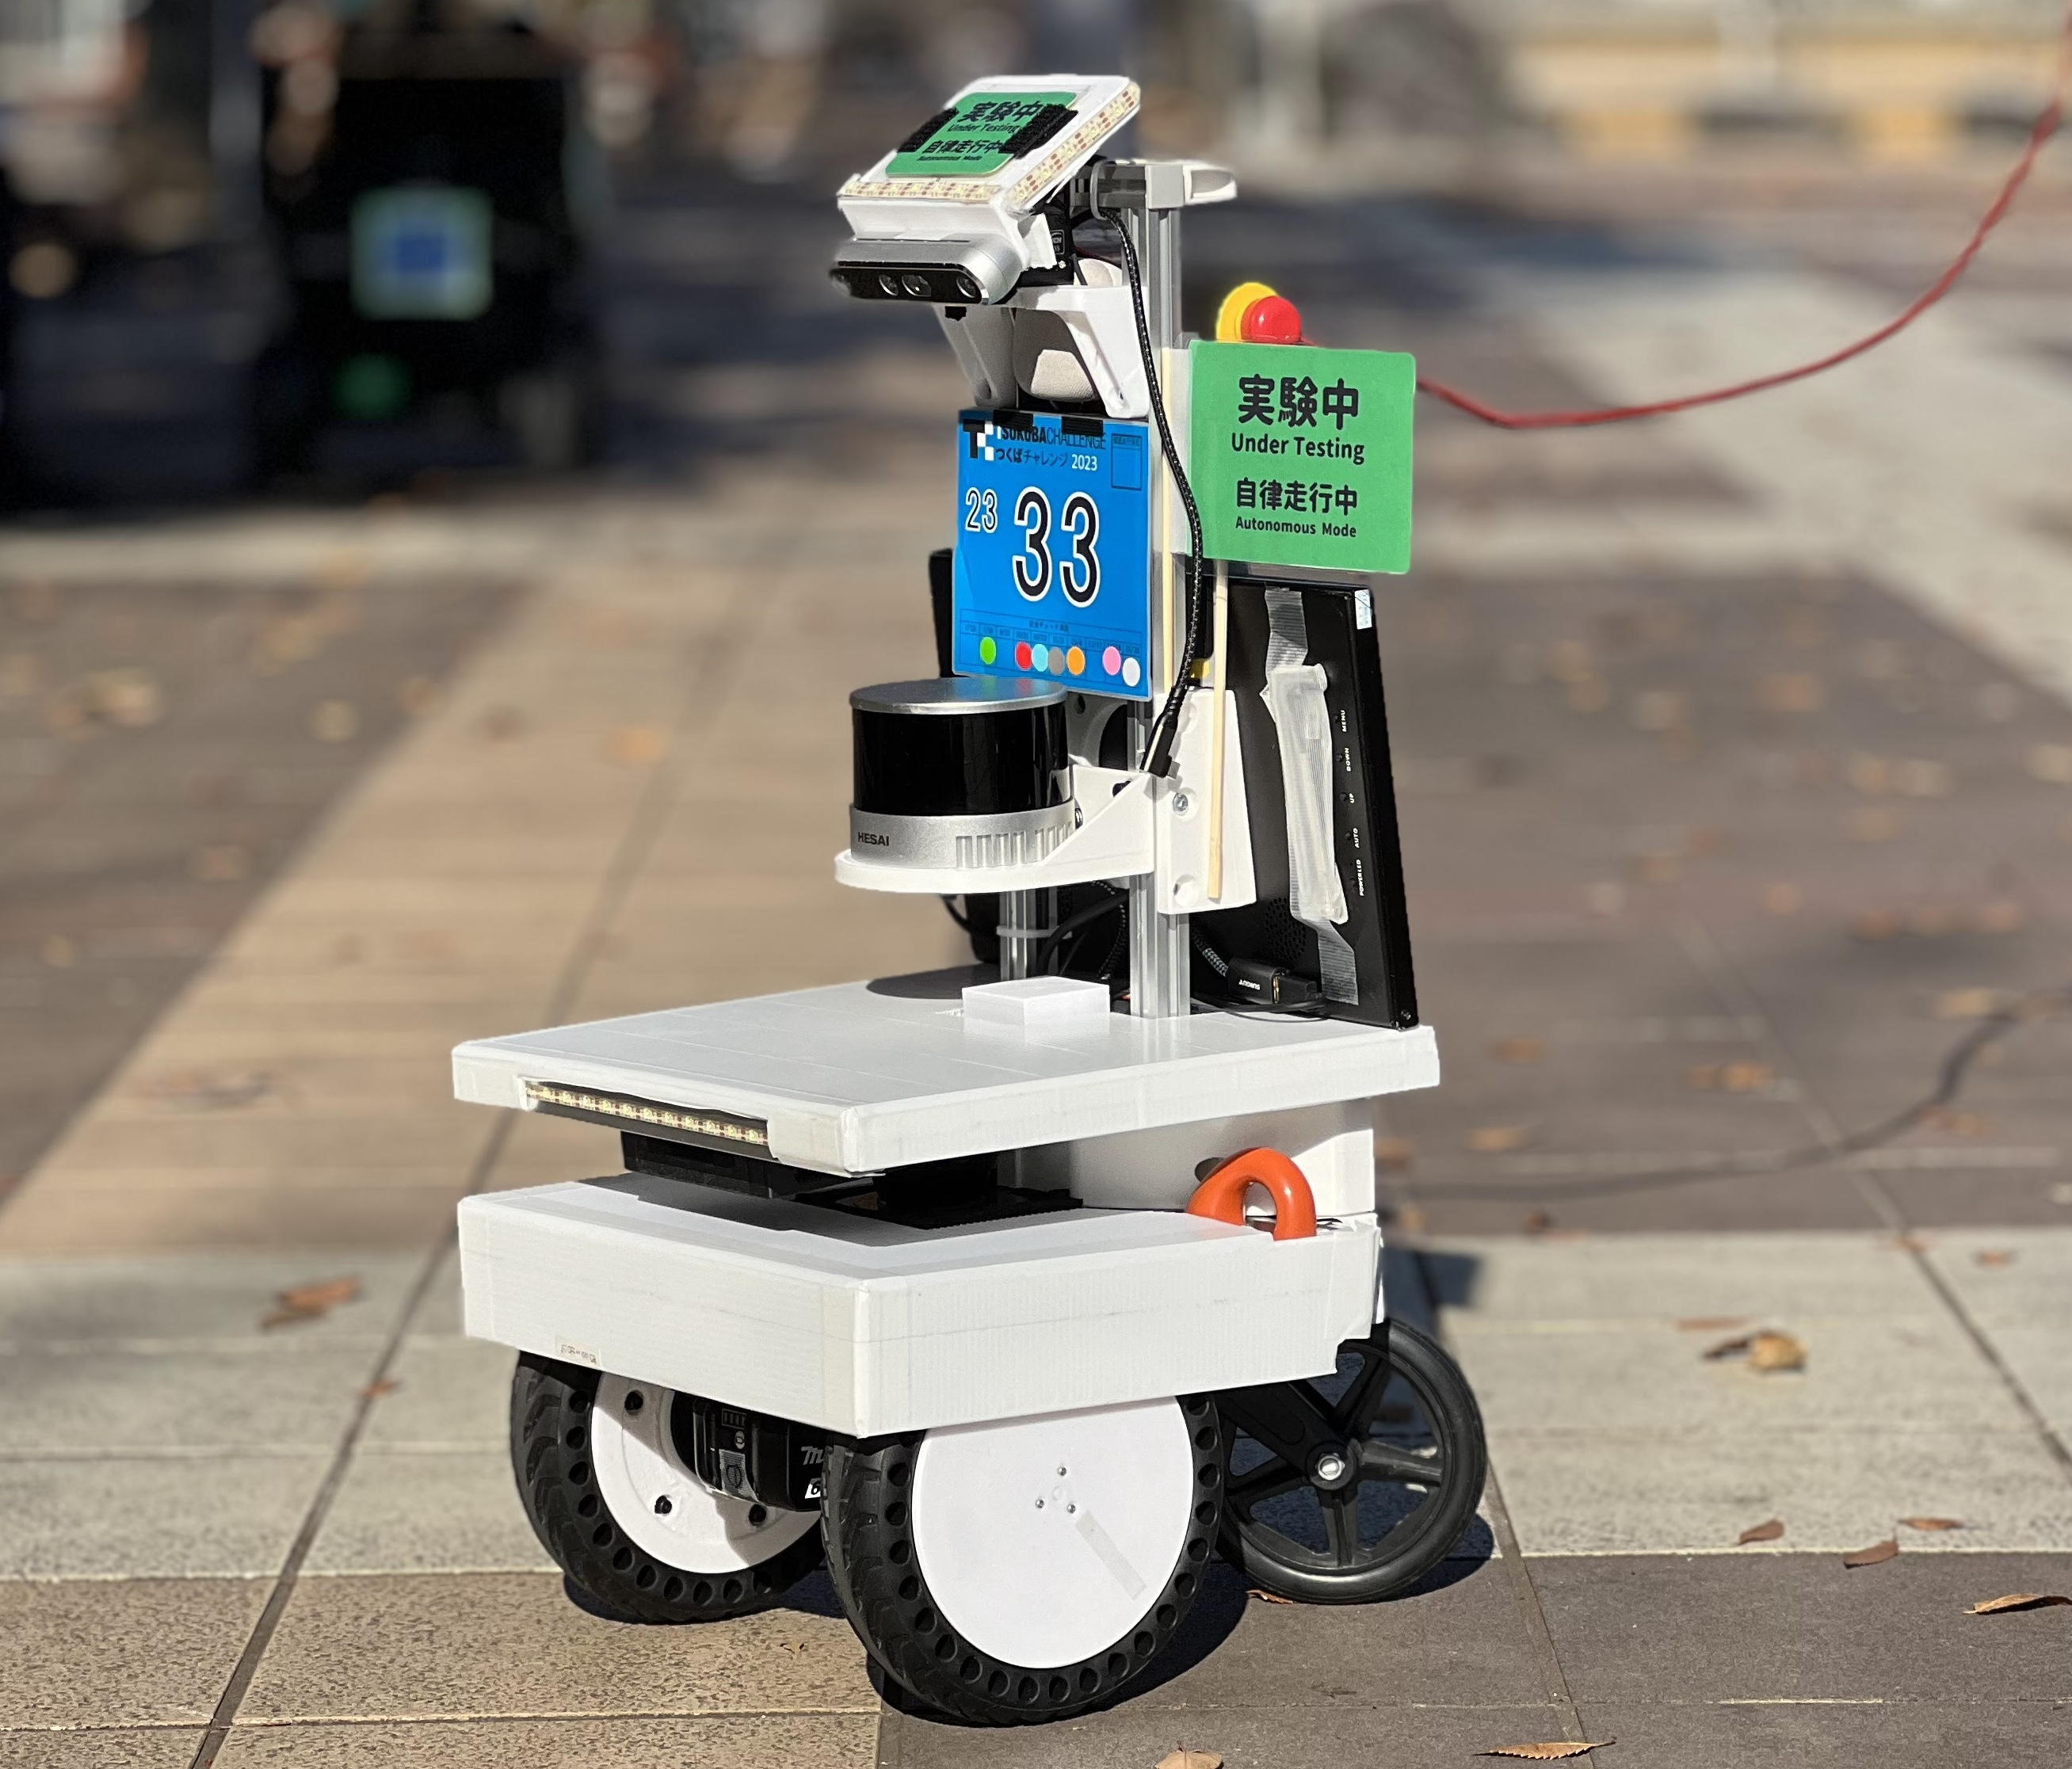
\includegraphics[width=75mm]{./picture/cub.jpg}
    \caption{Cub}
  \label{fig:cub}%\vspace*{-2mm}
\end{figure}

%\begin{equation}
%P(B\mid A) = \frac{P(A\mid B)P(B)}{P(A)}
%\end{equation}

%\begin{itemize}
%\item 第1の項目
%\item 第2の項目
%\end{itemize}

\section{ハードウェア}
%(設計思想とシステム構成:田中)
本章では開発した小型ロボットCubのハードウェアについて述べる。
まず出場にあたり、放課後活動として開発する自分たちの環境や条件に合わせてロボットの要件を下記のように設定した。

\begin{itemize}
\item (当然)つくばチャレンジ出場要件を満たすこと
\item 家庭の玄関で保管できるサイズ:400x400mm以内
\item 電車で一人で運搬できること:重量15kg以内、キャリーカートで運べる高さ(800mm以下)
\item ROS等State of the artな技術を学習でき、モダンな開発手法にマッチしたアーキテクチャ
\item 電源管理・デバッグ等、現地開発しやすい構成
\item 入手性やコスト面で有利な扱いやすい部品を使う(公式のデバイス貸し出しプログラムも積極活用)
\item 安全面や雨天等を考慮し、できる限り部品の露出を避けるカバーを設けること
\end{itemize}

\begin{figure}
    \centering
    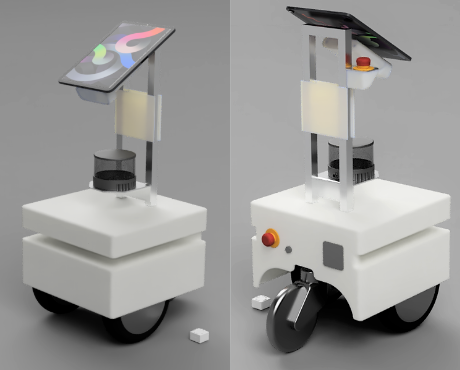
\includegraphics[width=0.8\linewidth]{picture/cub_first-design.png}
    \caption{Cubの初期デザイン外観\\タブレットは最終的に撤去し背面にモニタを搭載した}
    \label{fig:first-design}
\end{figure}

図\ref{fig:hw-layout}と図\ref{fig:hw-system}に具体的なハードウェアの構成を示す。なお、GPSやカメラのチルト用サーボモーターなど、今回は使用していないが将来のために搭載されているデバイスもある。

\begin{figure}
    \centering
    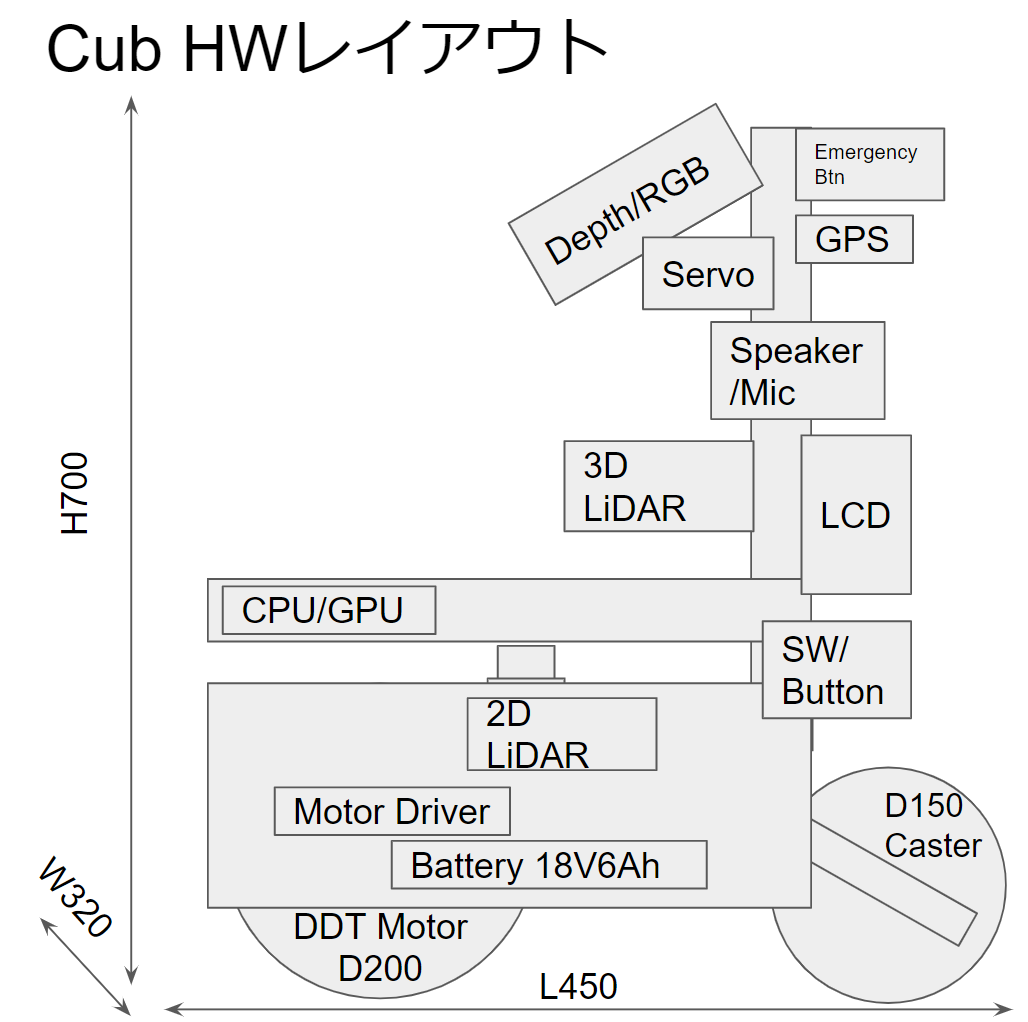
\includegraphics[width=0.8\linewidth]{picture/tc2023CubHWLayout.png}
    \caption{ハードウェアレイアウト図}
    \label{fig:hw-layout}
\end{figure}

\begin{figure}
    \centering
    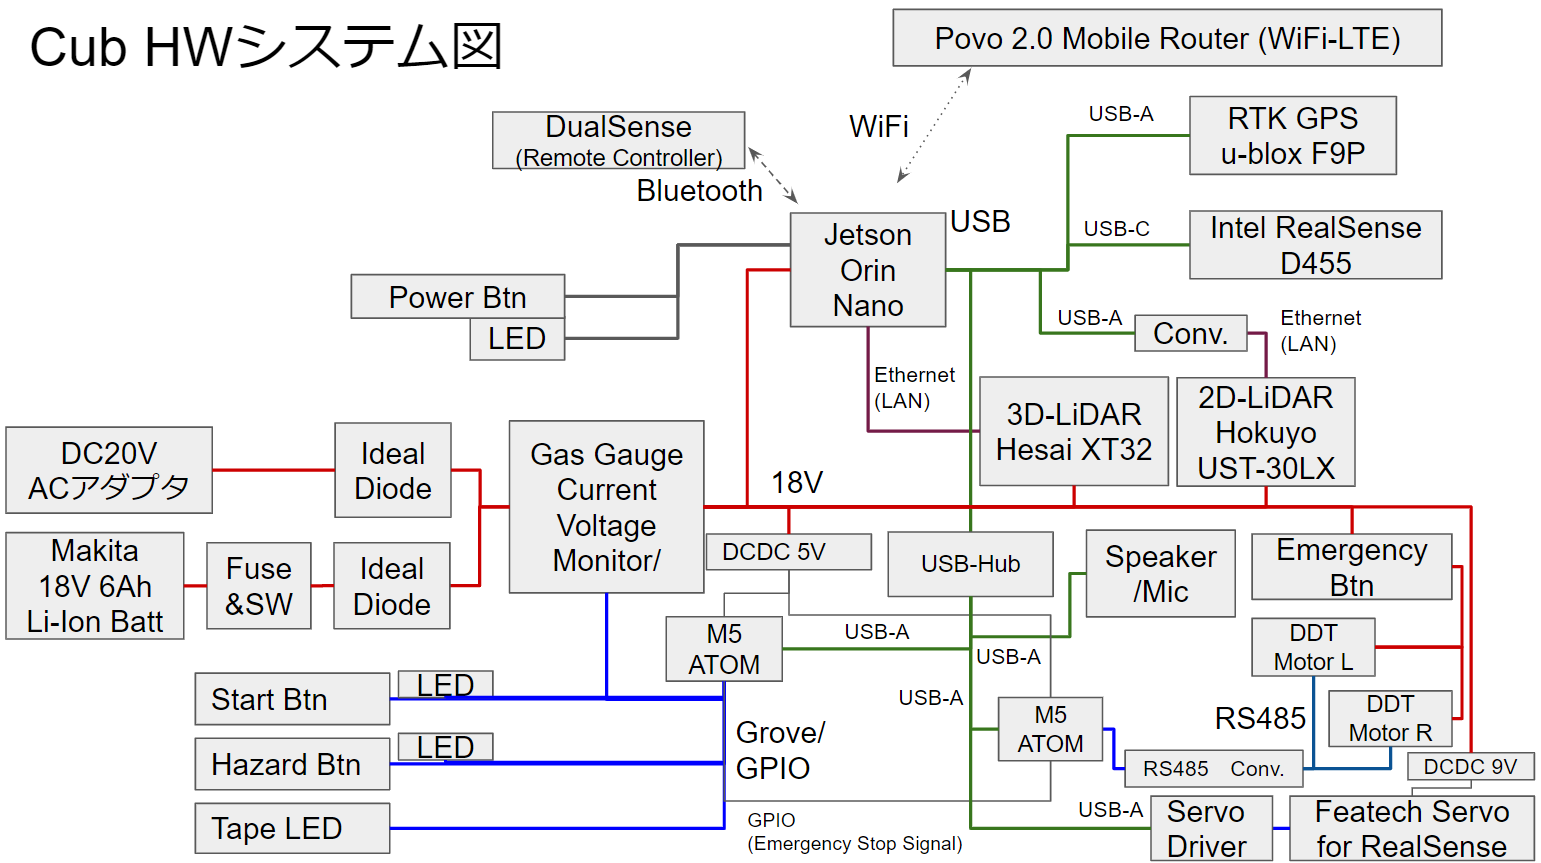
\includegraphics[width=1.0\linewidth]{picture/tc2023CubHW.png}
    \caption{ハードウェアシステム図}
    \label{fig:hw-system}
\end{figure}

今回初出場であったためサイズ制限等は設計自由度を下げる要因となり設計面では厳しかったが、放課後活動として活動場所が市民館等となってしまうことや電車運搬となること、保管が自宅になってしまうことなどから必要な制約となった。
しかし結果的にはコンパクトなサイズで片手で持てる重量を実現でき、安全面でも見た目の恐怖感の面でも優位性のある、比較的かわいらしいデザインとすることができた。
以上の要件から、下記特徴を持つロボットを設計した。

\begin{itemize}
\item 前輪駆動型対向二輪ロボットとし、キックボード用車輪+ダイレクトドライブモーターと車いすキャスターを用いたコンパクトな3輪構成
\item 小型LinuxPC(Jetson Orin Nano)を内蔵しLiDARやカメラ・緊急停止ボタン等のみを上部に搭載した低背・低重心なハードウェアレイアウト
\item 開発やメンテナンス性で優位な起動中の電源給電・電池交換(ホットスワップ)可能な電源構成
\end{itemize}

今回安価なRS485コマンド通信タイプのダイレクトドライブモーターDDT M0601C 111\cite{ddt}を電動キックボード用の車輪に内蔵して使用したことで非常にコンパクトな台車を構成することができ、十分なスピードやトルク・応答性を確保することができた。制御系にはM5Stack社ATOM Matrix\cite{atom}を使用し、既存のDDT M0601C用ライブラリを利用できたほか、PlayStation5用無線コントローラーDualSenseともBluetoothにて直接通信することで早期の制御系立ち上げを行うことができた。バッテリーには電動工具用の汎用的な18Vリチウムイオン電池を使用することで入手性や容量・ピーク電流・耐久性などの性能面で十分なパフォーマンスを発揮することができた。また、理想ダイオード\cite{diode}を用いたホットスワップ回路を用いることで電源のAC給電~バッテリー切り替え・交換をシャットダウン無しに行うことができ、開発効率を向上できた。メインCPUについてはNVIDIA Jetson Orin Nano\cite{jetson}を使用することでスムーズなROSでの開発を可能とし、小型軽量かつ将来のGPU利用も含め十分な性能を確保した。フレームや構造部材はミスミのアルミフレームと3Dプリンタ部品を使用し、安価で頻繁な設計変更を可能とすることで短期に新開発の駆動系を完成させることができた。センサとして障害物回避やナビゲーション用のLiDARには3DのHesai XT32(無償貸与)、2Dの北陽電機URM-40LC-EW(無償貸与)、距離センサとしてIntel RealSense D455(中古品購入)を搭載した。つくばチャレンジの過去のレポートやデバイスの動向を調査しながら、参照情報の多いモダンな汎用部品を多用することで学習や立ち上げにかかる時間を短縮し、比較的ミニマルな構成で小型な屋外自律移動ロボットを実装・構築することができた。

\begin{figure*}[h]
  \centering
  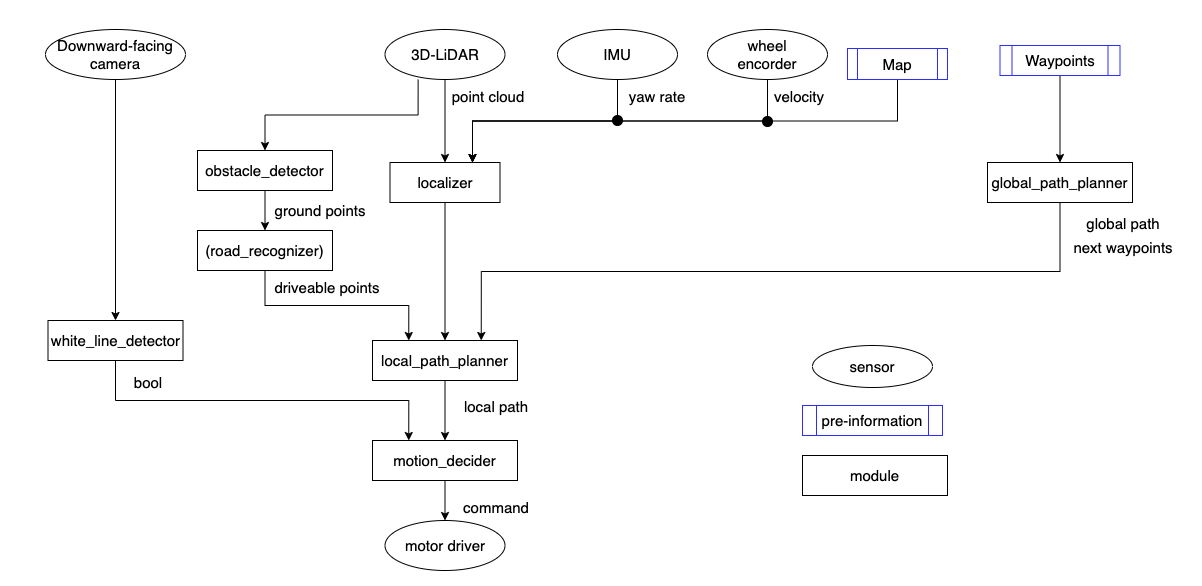
\includegraphics[width=160mm]{./picture/system_architecture.png}
    \caption{System architecture}
  \label{fig:system_architecture}%\vspace*{-2mm}
\end{figure*}

\section{ソフトウェア}
本章では、作成したナビゲーションシステムのソフトウェアについて記述する。
図\ref{fig:system_architecture}はシステム図である。

システム全体のフレームワークとしてはROS1 Noetic\cite{ros}を使用し、内界センサ(IMU・ホイールのオドメトリ)の情報と3D-LiDARのスキャン点群と点群地図によるNDT\cite{NDT}スキャンマッチングの情報を拡張カルマンフィルタで統合し自己位置推定を行った。
また、3D-LiDARの計測点群から走行可能領域を認識し、事前に設定したウェイポイントを障害物を回避しながら順番に巡回することで自律移動を行う。

\subsection{内界センサ・自律航行系の構成}
% @takagi.h  @永谷 智貴\\
% ROSやM5Stackを使うコツや苦労なども
自己位置推定・自律航行を行うためのオドメトリ取得に使用した内界センサデバイスを (表\ref{tab:odometory_imu_devices}) に示す。
\begin{table}
\centering
\caption{内界センサとして使用したデバイス}
\label{tab:odometory_imu_devices}
\scalebox{0.75}{
\begin{tabular}{llc}
\hline
型番& ベンダー& 機能\\
 M5Atom& M5Stack& オドメトリ取得及びモーター制御\\
 DDT M0601C 111& Direct Drive Tech& モーター・エンコーダ\\
 BNO055 & Bosch& IMU\\
\hline
\end{tabular}}
\end{table}

コマンド通信タイプのモータードライバからの回転角情報を活用し、既存のArduinoライブラリ\cite{ddt_motor}を用いてM5Atom側で計算、速度制御及び位置情報を取得しオドメトリ計算を行った。
当初はモータードライバの速度情報を元に積分によるオドメトリ計算を行っていたが、誤差蓄積が大きく使い物にならなかったため、位置情報を元に計算する方法に切り替えた。またYaw角の精度向上のためIMUを追加しカルマンフィルタによるジャイロオドメトリで位置・方向ともに自律走行が可能な精度を達成した。
ROS1のシステムへの合わせこみに関しては、rosserialライブラリ\cite{rosserial}を活用した。

\subsection{大域的経路計画}
% @Tshibuya (サポート @永谷 智貴 )
今回作成したDijkstra 法\cite{dijkstra}による大域的経路計画について述べる。
使用する3次元点群を参照し、事前に分岐点や通過したい地点などにウェイポイントを設定し、
各ウェイポイント間の距離をDijkstra 法のコストとすることで、指定したウェイポイントを最短で通過するような経路を生成する。

% ---To 永谷さん ウェイポイント設定について書くのもありかなと----
ウェイポイント設定には、RVizとChatGPTを活用した。まずRVizにクリック対象の地面とする十分に大きな空のMapと三次元地図とを配置し、Publish Point機能で座標をTopicとして出力するよう設定した。このTopicをスクリプトによりウェイポイントを表すyamlファイルに保存し利用した。この仕組みにより、座標の手打ちを避けられ手間を削減出来た。これに必要なスクリプトは全てChatGPTを用いて要件・仕様のテキストからコードを生成したものを僅かに手直しして実現したものであり、開発の手間・時間も削減出来た。

\subsection{局所的経路計画}
% @Tshibuya (サポート @永谷 智貴 )
今回利用した局所的経路計画について述べる。
まず、3D-LiDARの計測点群から高さ情報を元に障害物に関する点群を抽出し、抽出した障害物に関する点群を用いて二次元の格子地図を作成する。
作成した周辺地図と推定した自己位置の結果、次に目指すウェイポイントの位置を元にState Lattice Planner\cite{state_lattice}を用いて、障害物にぶつからないような軌道を生成しすることで、安全に各ウェイポイントを巡回する。

\subsection{白線・物体検出}
%@yoshitake\\
ここでは白線・物体検出の実装と本番での稼働状況について記述する。検出に使用したデバイスを (表\ref{tab:white_line_devices}) に示す。

\begin{table}
\centering
\caption{白線・物体検出に使用したデバイス}
\label{tab:white_line_devices}
\begin{tabular}{llc}
\hline
型番& ベンダー& 機能\\
 Realsense D455& Intel& 光学カメラ、深度カメラ\\
 Jetson Orin Nano& Nvidia& 物体検出\\
Windows PC& HP& 開発・デバッグ環境\\
\hline
\end{tabular}
\end{table}

% memo: 日本語はともかく書きたいことをとりあえず書く。\\

白線・物体検出は、RealsenseとJetsonおよびWindows PC上のPythonプログラムによって行った。RealsenseはSDKのPythonラッパーであるpyrealsense2を使用することでRGB画像、深度画像、IMU情報を取得することができる。RGB画像は各色8ビット、深度画像は16ビットとし、それぞれを位置合わせした状態で受け取る。ホスト側の処理能力を考慮して、リフレッシュレートは5 Hzとし、解像度は最大の1280 $\times$ 720 pixels $^2$とした。単純に取得した深度画像は欠損が多く、そのままでは使いにくいので、SDKのPost Processing機能であるHole Fillingによって補間している。なおIMUの情報は今回は使用していない。

白線および物体の検出にはRGB画像を用いた。視野の下半分のみ注目領域とし、入力画像をトリミングした。細かいテクスチャにより県検出精度が落ちないようにガウシアンぼかしを適用した。画像内から白い領域だけを抽出するために、RGB色空間からHSV色空間に変換し、$0 \leq S \leq 50$かつ$200\leq V \leq 255$のピクセルのみを255とし、残る領域を0とするマスク画像を作成した。OpenCVのCanny法によってマスク画像から輪郭を抽出し、同様にハフ変換にて直線を検出した。ハフ変換のパラメーターの一例として次を使用した。$\mathrm{rho}=1, \mathrm{theta=np.pi} / 180, \mathrm{threshold}=100, \mathrm{minLineLength}=200, \mathrm{maxLineGap}=20.$ 白線に対して機体が正対していることを前提とし、視野内で水平な直線だけを抽出するために、画像の横方向を角度$\phi=0^\circ$として、水平なもの ($-10^\circ \leq \phi + 180^\circ \times n \leq 10^\circ$) のみを残した。最後に白線の中心座標を算出し、深度画像を参照することで、白線の検出と白線までの距離を取得した。

物体認識はUltralytics社のYOLOv5\cite{yolo}を使用し、事前学習モデルはyolov5sを使用した。特に変更は加えず、そのまま使用した。十分に遠い物体を検出から除外するために、画像全体に対して検出された矩形の面積が1/64以上ある物体のみを残した。検出された矩形領域の中心8$\times$8 pixels$^2$に対し、深度画像から平均距離を取得した。物体の矩形領域全体の平均を計算すると、背景に引っ張られて正しい距離を取得できない。

実機にRealsenseを取り付け、Windows PC上でPythonを実行しながら検出のテストをしたところ、タイルの継ぎ目などで白線の誤検出が発生したので、目的の白線に接近した場合のみ検出結果を有効にする必要が分かった。しかしながら、本走行までに自律移動が可能な状態に至らず、Jetson Orin Nanoを使用した完全な状態での動作確認およびパラメーターのチューニングまで完了しなかった。今後、継続的に開発が必要な要素となっている。


\section{つくばチャレンジEXに向けた改修}

今回初出場ということもあり、できるだけ現場経験値を積むためつくばチャレンジEXにも参加することにした。特につくばチャレンジ with PLATEAUは地図データの活用の点で過去の蓄積のない自分たちにとっても得るものが大きいと考え挑戦することとした。

\subsection{PLATEAUデータの変換}
G空間情報センターのPLATEAUつくば市データ\cite{pltsukuba}をダウンロードし、PLATEAU SDK for Unity\cite{plateau_unity}を使ってOBJデータを作成、その後PCL mesh2pcd\cite{pcl_mesh2pcd}を使いOBJから点群データに変換した後で座標の不整合をCloud Compareというツールで修正してROS用の点群地図ファイルを作成した。当初つくばチャレンジEX with PLATEAUのチュートリアル\cite{tcexpl}を参考にFMEというデータ変換ソフトウェアを利用しようとしたが、ライセンスの取得に時間がかかることが分かったため使用できなかった。Unity上では不要なデータを細かいオブジェクト単位で編集・削除することができるため、結果的にはロボット視点で不要なデータをすべて削除することができ、必要最低限のデータセットを構築することができた。
\begin{figure}
    \centering
    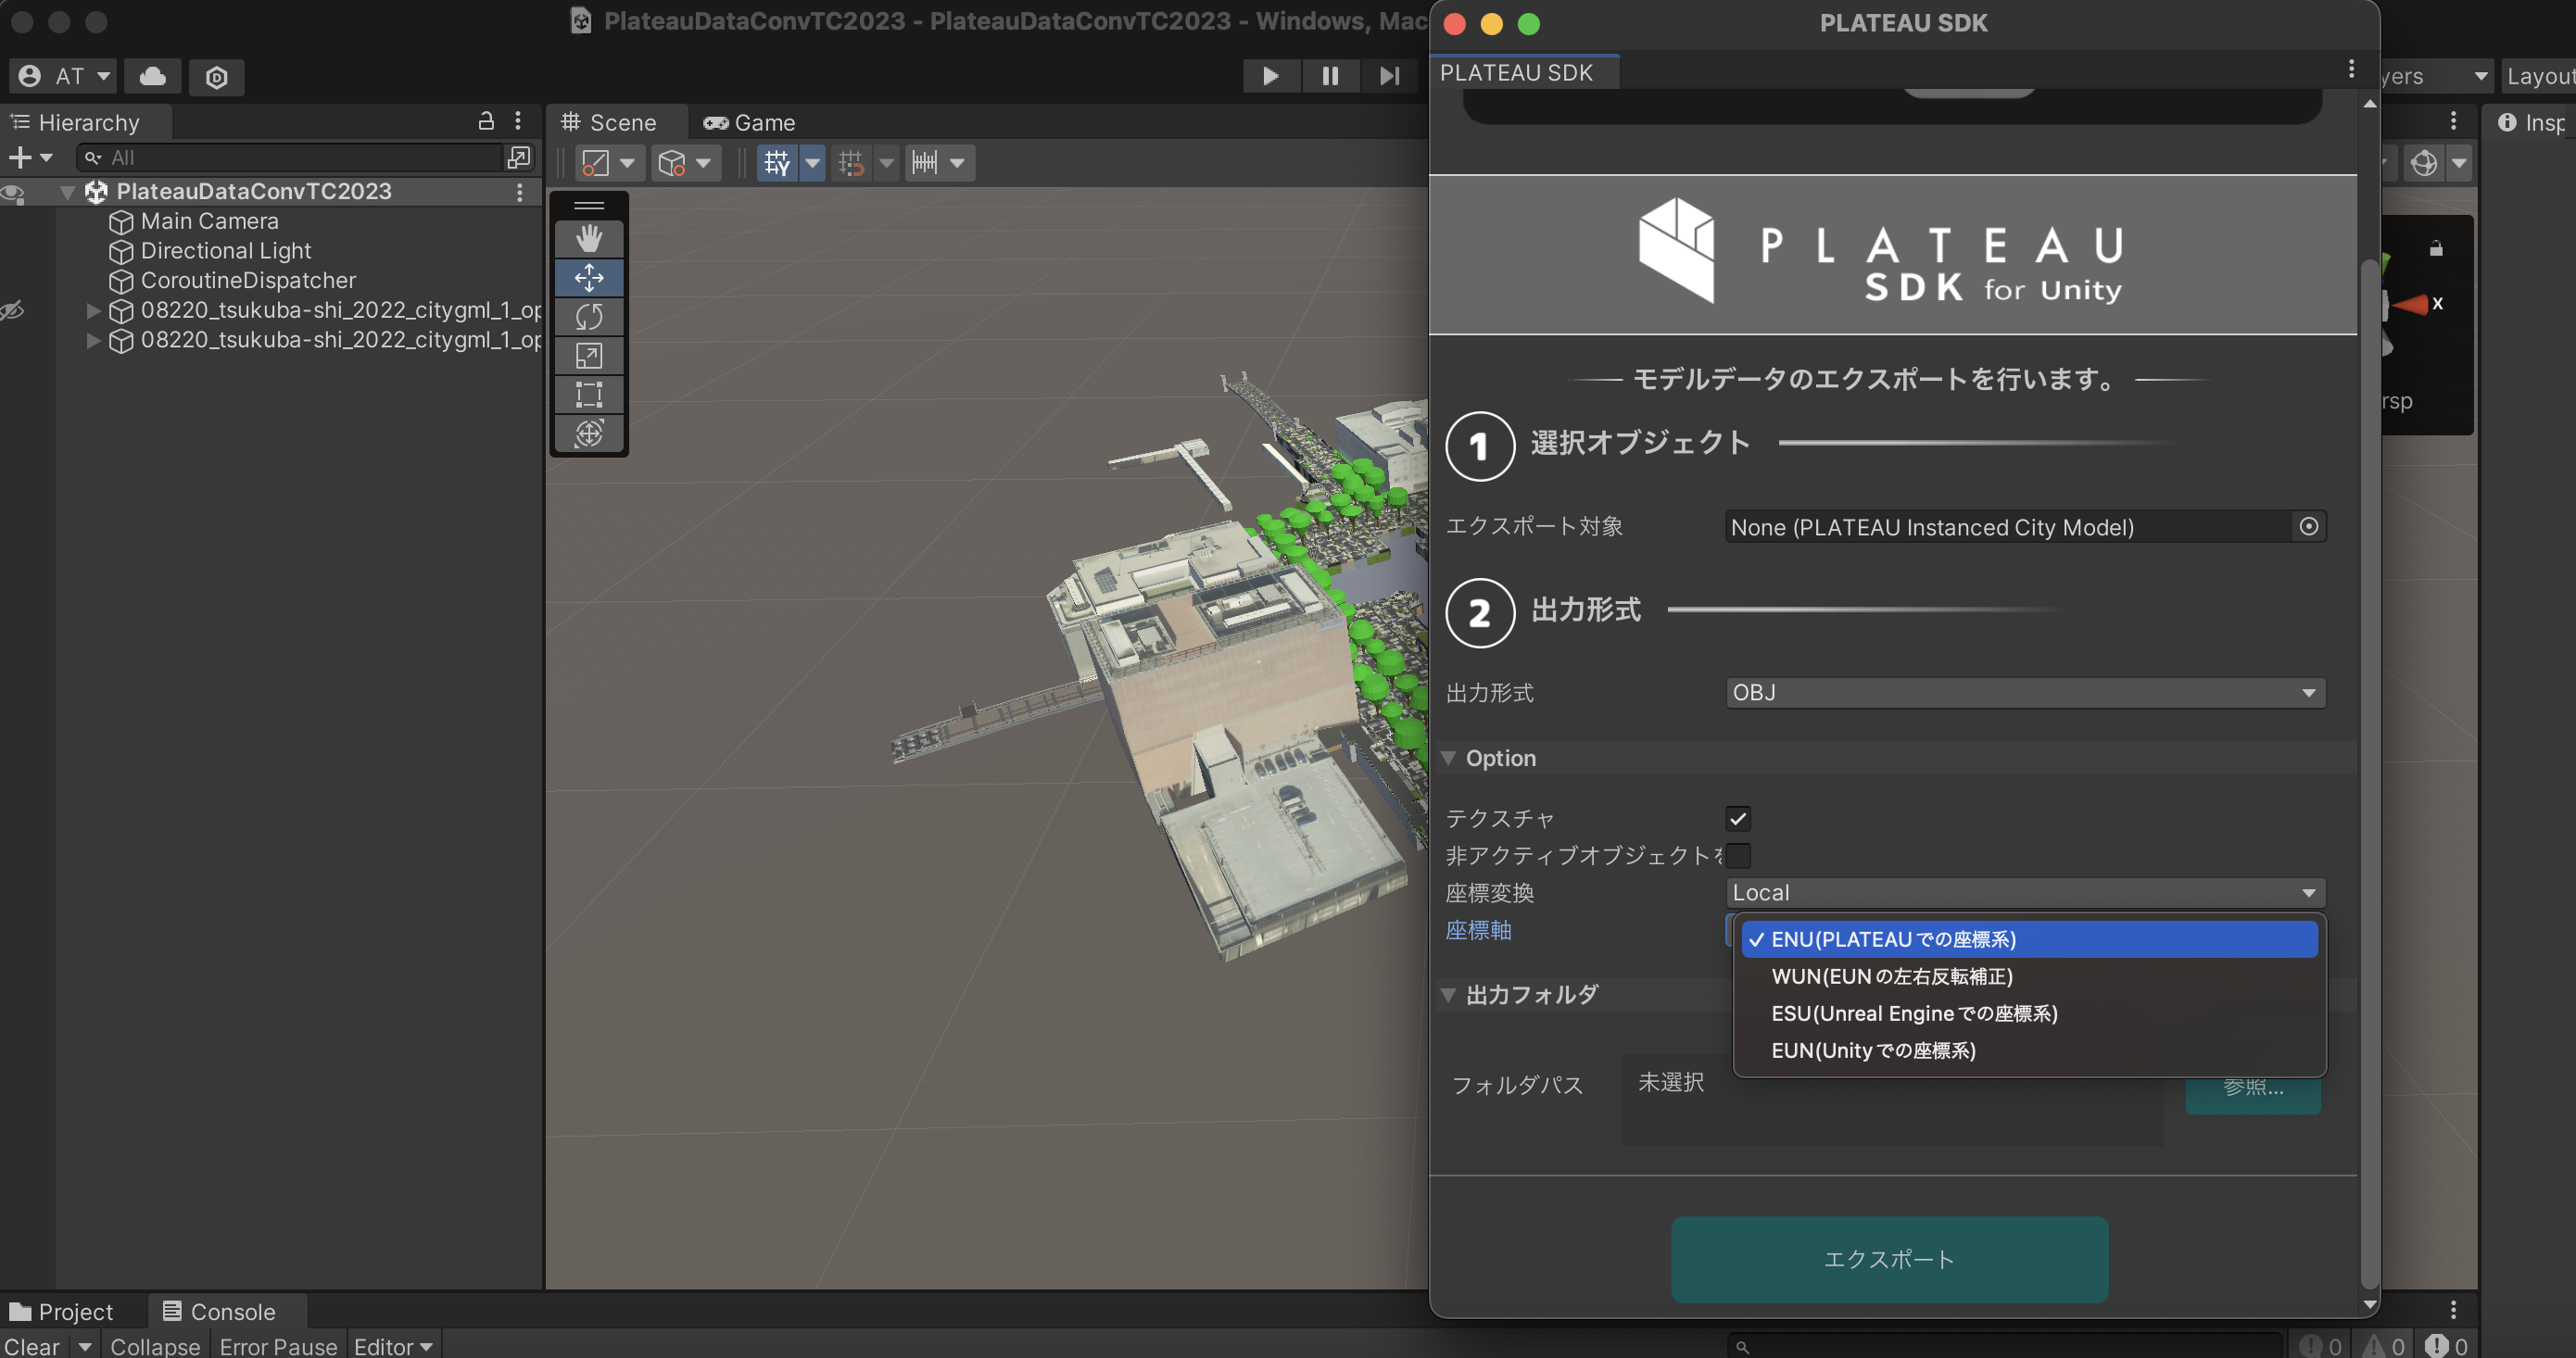
\includegraphics[width=0.8\linewidth]{picture/plateau_unity.png}
    \caption{PLATEAU SDK for Unityでのデータ加工}
    \label{fig:plateau_unity}
\end{figure}

\subsection{ROS対応}
% @Tshibuya
PLATEAUデータから変換した点群データは、左右反転した状態であったため、点群データに変換後にcloudcompareを用いて修正を加えた。
また、変換した点群データの点密度が低かったため、3D-LiDAR点群とのマッチングが取れない場面が多く見受けられた。
それを対応するために、変換した点群を複数コピーしそれぞれ数mmずらして重ね合わせたものを一つの点群地図として扱うことで点密度を向上させ、スキャンマッチング精度の向上を図った。

\section{実験結果}
% @yoshitake ( @takagi.h , @Tshibuya )\\
% 簡単に本走行とつくチャレEX2回まとめたものでOK、データもあるといいが基本は写真、感想と考察や今後の改善点も\\
\begin{figure}
    \centering
    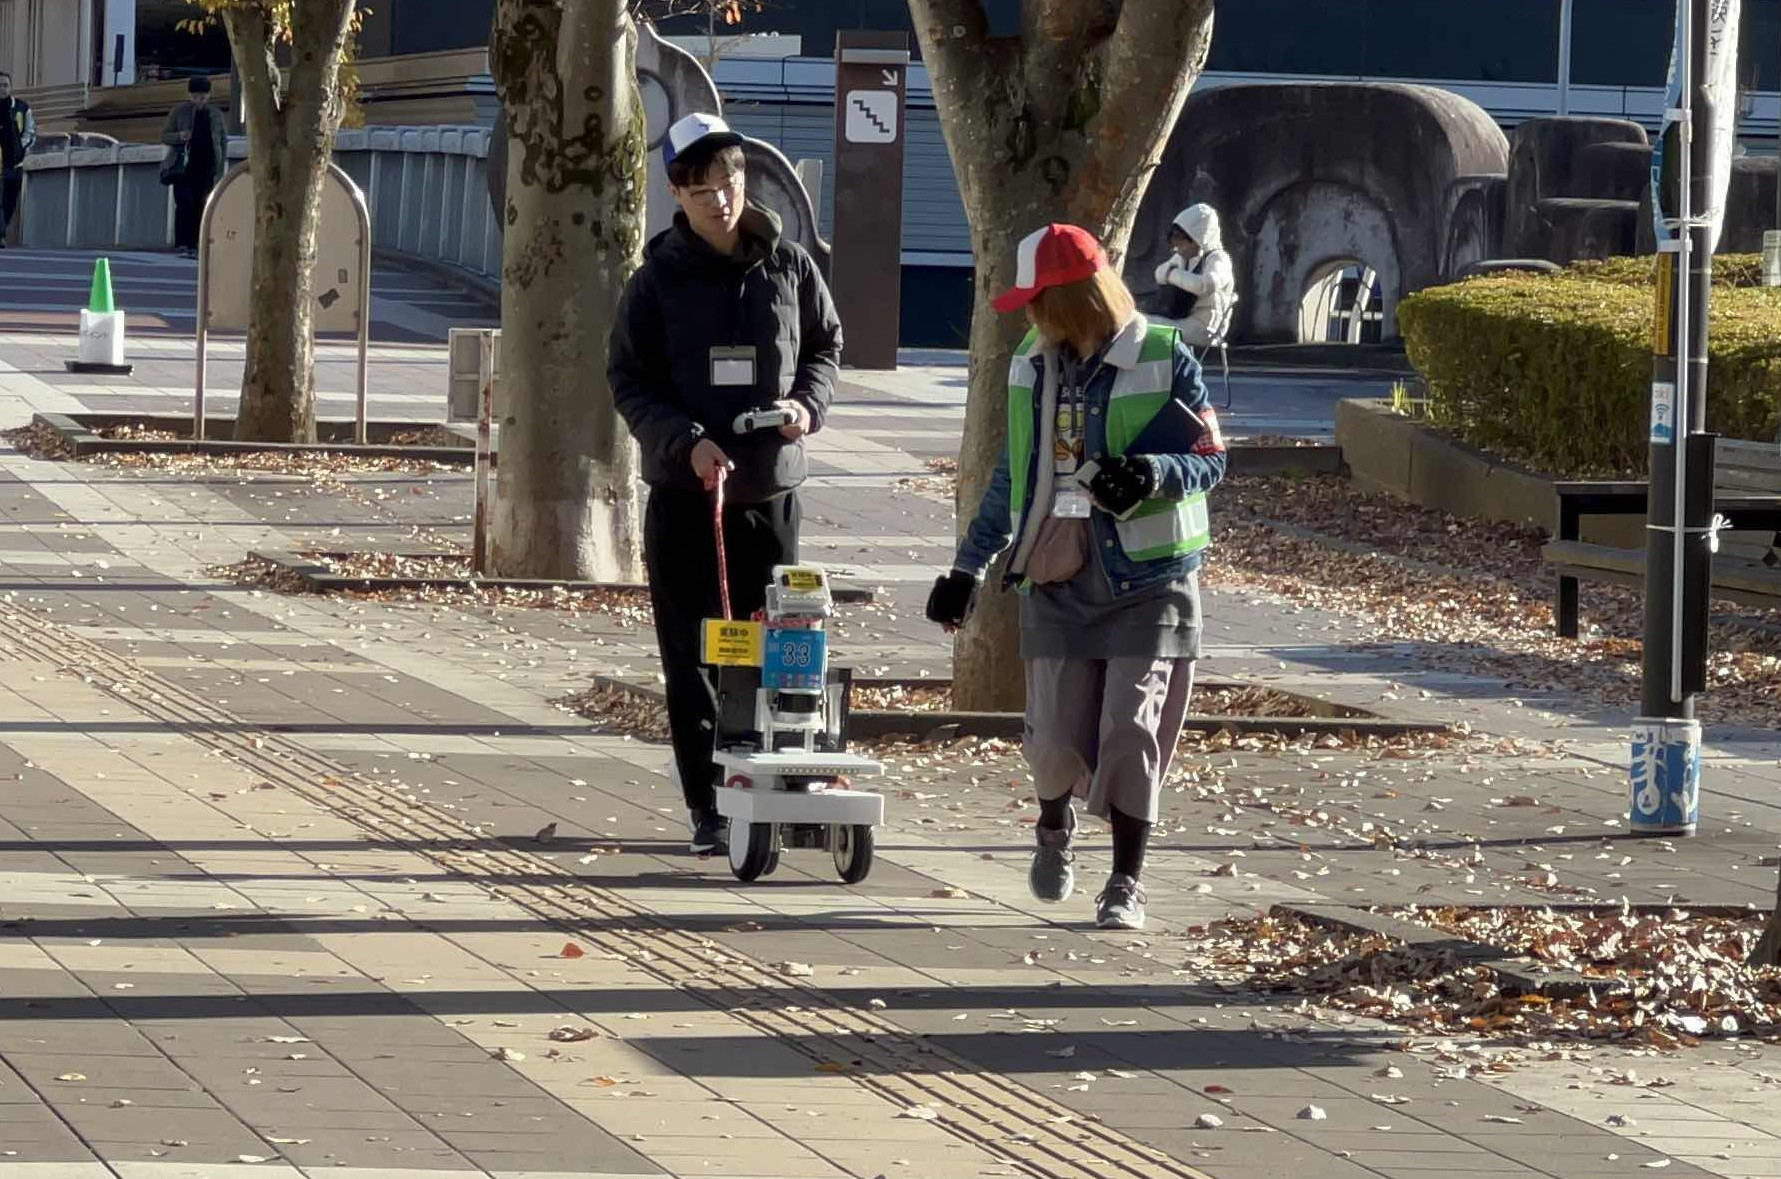
\includegraphics[width=0.8\linewidth]{picture/tc2023exp.jpg}
    \caption{つくばチャレンジEX with PLATEAUの様子}
    \label{fig:plateau_exp}
\end{figure}

本機体は表\ref{tab:cub_entry_events}のとおり、本走行の1回とつくチャレEXの2回に参加した。それぞれの結果と考察や感想を記述する。
\begin{table}
\centering
\caption{Cub参加イベント (記録認定のあるイベントのみ)}
\label{tab:cub_entry_events}
\begin{tabular}{ll}
\hline
日程& イベント名\\
 8/17--18& つくばチャレンジEX\\
 &@イーアスつくば\\
 11/19& 本走行\\
 12/3--4&つくばチャレンジEX with PLATEAU\\
& @つくばセンター広場\\
\hline
\end{tabular}
\end{table}

はじめに、各イベントでの結果を記す。「つくばチャレンジEX@イーアスつくば」および「本走行」では、スタートすることができなかった。「つくばチャレンジEX with PLATEAU@つくばセンター広場」では、数十メートルの自律移動に成功したものの、途中でコースアウトにより緊急停止、棄権・失格となった。\\

各イベントに対し、考察や感想を含めて詳細に記す。「つくばチャレンジEX@イーアスつくば」では、ハードウェアはおおむね完成しており、走行装置をラジコン操作できる状態であったが、ソフトウェアの開発が追いついておらず、LiDARなどのデバイスの立ち上げやROSの完全な構築ができていなかった。そのため出走できずやむなくリタイアとなった。感想としては、今年初めて参加した本チームから見て、他の参加チームの機体の完成度が驚くほど高く、ノウハウの蓄積の優位性を痛感した。特に、施設の入場口付近で4台の機体がお見合いになる難しい状況に、各自が自律的に回避や後退を行って走行を続ける場面が印象的で、自律移動を行うことのハードルの高さを感じた。

「本走行」では、事前に一定距離の自律移動はできるようになっていたものの、直前のメンテナンスが原因でスタートラインを越えることなくタイムアップでリタイアとなった。本来であれば、ナビゲーションや自己位置推定を担当するJetsonとモーターを制御するM5Stack相互に指令やオドメトリをやり取りするが、直前にM5Stackのプログラムを書き換えたことで両者の接続が不安定になりスタート後正常動作できなかった。このミスの背景には、システム全体の完成度が上がっていないために、エラーに対して素早くリカバリーする体制が整っていなかったこともあった。

\begin{figure}[h]
  \centering
  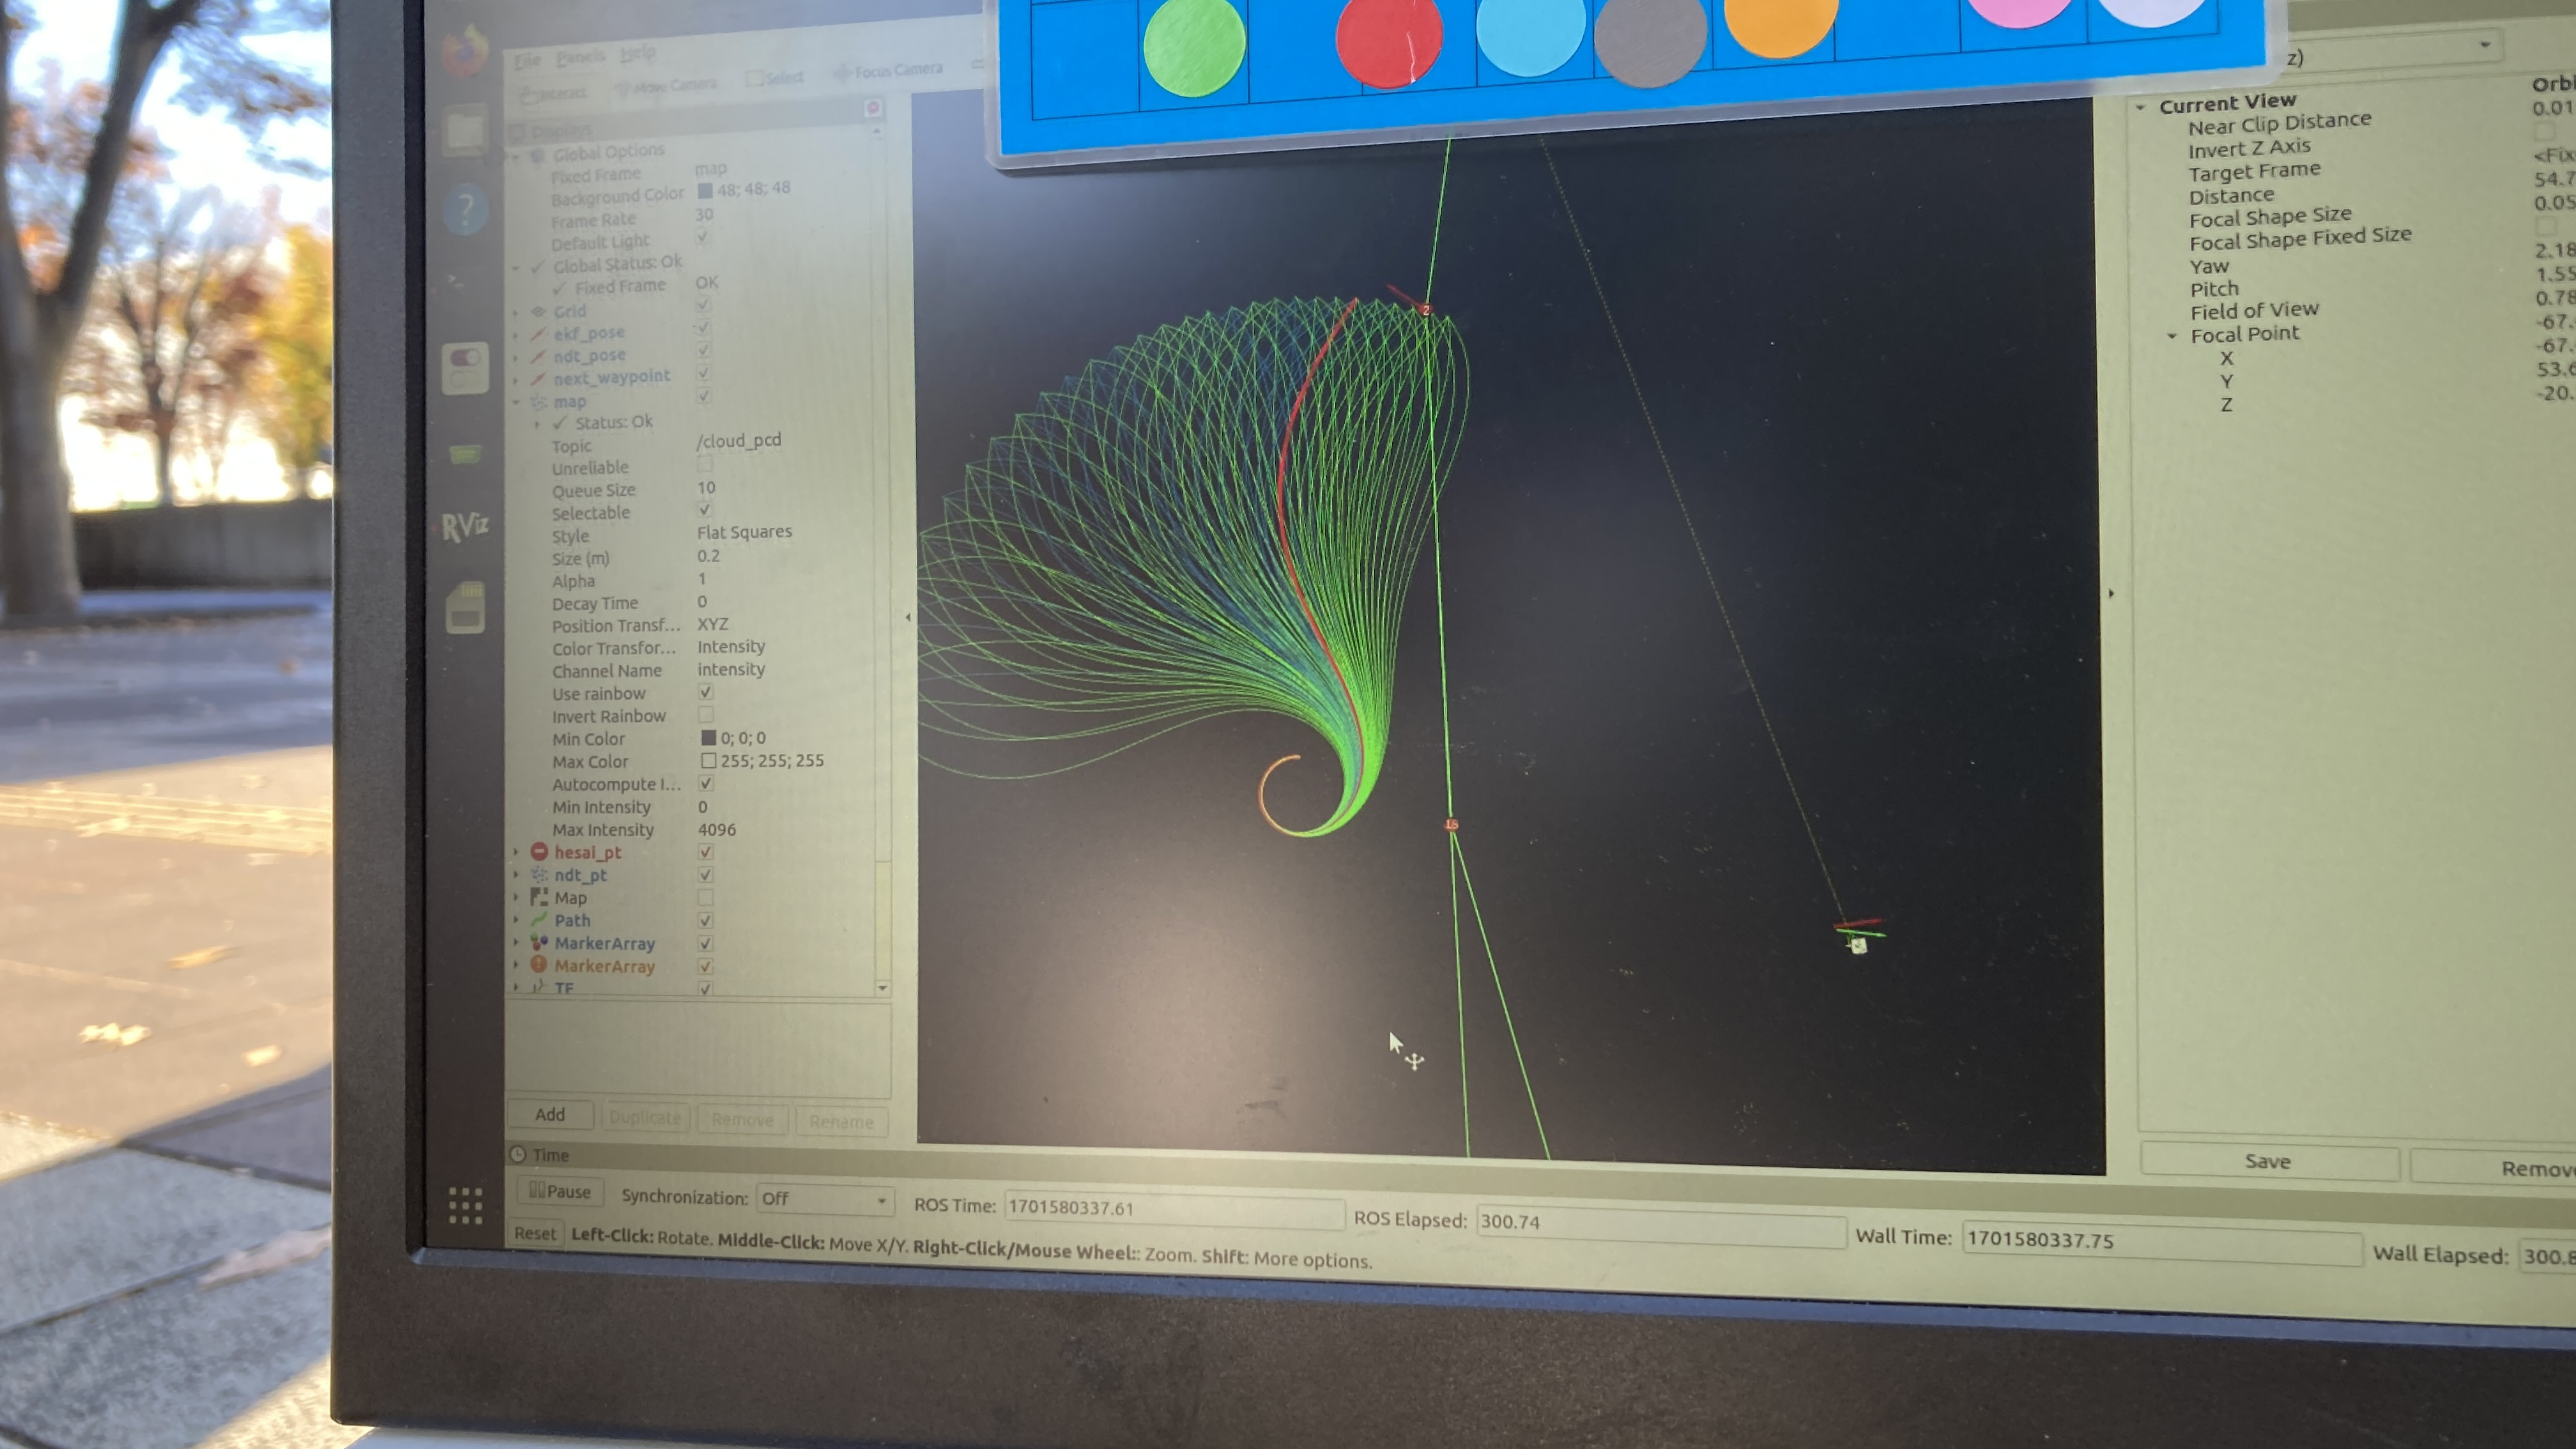
\includegraphics[width=80mm]{./picture/guruguru_path_plan.jpg}
    \caption{EX走行失敗時の経路生成の様子(原因解析中)}
  \label{fig:guruguru_path}%\vspace*{-2mm}
\end{figure}

「つくばチャレンジEX with PLATEAU@つくばセンター広場」では、各デバイスは正常につながり、自律移動も開始できたが、経路生成の異常が発生したために、コースアウトすることとなった。その時の経路の様子を図\ref{fig:guruguru_path}に示す(緑線:候補軌道、青線:衝突回避軌道、赤線:選択軌道)。なお、まだ原因は特定できておらず、継続的に調査を進める必要がある。

\section{今回活用できなかったアイテム}
今回つくばチャレンジ初出場にあたり、公式の貸し出しプログラムを最大限活用させていただいた。しかし、実際の開発においては時間制約やスキル、またシステムとの相性なども含め十分に活用できなかったアイテムが多数発生してしまった。ここに原因を含めて紹介しつつ、無償提供していただいたことへの心からの感謝と十分活用できなかったことへのお詫びの気持ちを表したい。

\begin{itemize}
\item 北陽電機様:Lidar「URM-40LC-EW」を貸与いただいたが、ROS向け設定で手間取り(結果的に単純ミスと判明)システム統合ができなかったこと、また3D LiDARでの障害物回避で走行自体はできたことから活用できなかった。今後エリア設定機能を使った衝突防止センサとして安全機能向上に活用したい。
\item マップフォー様:3次元SLAMソフトウェア「MAP IV Engine Cloud」のライセンスを貸与いただいたが、結果的にはチーム内経験者の知見を活かし全体をROS1で開発することとなり、また事前配布された地図やPLATEAUを活用したことから使用できないままに終わってしまった。次回以降は改めて3DSLAMで独自地図を作成したい。
\end{itemize}

\section{おわりに}
今回社会人サークルとして初めてつくばチャレンジに参加したが、とても楽しく参加でき学びも非常に大きかった一方、実際にはロボット開発だけでなく当初想定上に開発環境や体制の構築に苦労した。なによりまずは開発場所の確保として近隣の市民館を利用したが会議室の予約が取れないといった初歩的なところからの苦労も多かった。また、チームメンバーも基本的にはなかなか普段会えないためリモート開発と集合開発を組み合わせたが、実機が1つしかないため最終的なすり合わせが結果的に現場での実験に依ってしまった点は開発の大幅な遅れにもつながった。これらの点は経験値不足からの点もあり、今後改善していきたい。
いずれにしても、今回既存のロボットを使わずに自作でコンパクトなロボットを開発できたことで、一般的なつくばチャレンジ出場ロボットより低コストかつコンパクトと思えるミニマルなものができ、家庭での保管や電車での移動にも対応するなど社会人チーム・放課後開発に向いたロボットの参考例をつくることができた。自分たちとしてもこれをバネに今後の出場や完走を目指すとともに、ぜひこれを読んでいただいた社会人の方・サークルのみなさんにも参考にしていただければ本望である。つくばチャレンジというリアルな実験と開発を通じて得られた実学的な学びは何物にも代えがたいということは最後に申し添えたい。

\section{謝辞}
応援してくれたサブメンバー福林さん、快く開発場所を貸していただいた川崎市立中原市民館・かわさき市民活動センターのみなさま、応援してくれたCoderDojo武蔵小杉の参加者のみなさん、そして背中を押してくれた家族へ心から感謝の意を表します。また最後に、つくばチャレンジという素晴らしい挑戦の場を企画・運営・支援いただいた運営委員会・スタッフ・つくば市のみなさまに心からお礼申し上げます。
% 参考文献
\bibliographystyle{junsrt}
\bibliography{myrefs}


\begin{comment}
以下、参考情報

\section{参考文献}
参考文献の参照例.
\begin{itemize}
\item NDTの参照例 \cite{NDT}
\item DDTMotorのArduinoライブラリ \cite{ddt_motor}
\item Rosserial Arduino Library \cite{rosserial}
\end{itemize}


\section{図表の挿入}
図表についても通常の \LaTeX と同じ方法を用いることができる.

\subsection{図について}
図の挿入は,通常\pkg{graphicx}パッケージによって行う(図\ref{fig:sample}).
クラスオプションにワークフロー(\code{dvipdfmx}等)を指定していれば,
各パッケージを読み込む際に何度も同じオプションを指定する必要はない.

\begin{figure}[t]
\centering
\includegraphics[width=3cm]{example-image-a}
\caption{図の例}
\label{fig:sample}
\end{figure}

\subsection{表について}
表の挿入は,\verb|\begin{table}...\end{table}|環境を使う(表\ref{tab:sample}).

\begin{table}[t]
\centering
\caption{表の例}
\label{tab:sample}
\begin{tabular}{llcc}
\hline
日本語 & Japanese & ほげほげ & ふげふげ \\
英語 & English & hogehoge & fugefuge \\
\hline
\end{tabular}
\end{table}


\section{Writing in English}
This paragraph shows an English sample.
There is no problem with writing your manuscript in English.
If you write in LaTeX, please use the distributed document class with the \code{english} option:
\begin{quote}
\verb|\documentclass[|\\
\verb|  platex,dvipdfmx,english]{rbproceedings}|
\end{quote}
\end{comment}

\end{document}